\section{Durchführung}
\label{sec:Durchführung}
\subsection{Kennlinienschar einer Hochvakuum-Diode}
Im ersten Teil der Durchführung wird eine Kennlinienschar einer Hochvakuum-Diode erstellt. 
Hierfür wird die Schaltung in Abbildung \ref{fig:ersteApparatur} ohne einen XY-Schreiber verwendet.
Dabei wird die Heizleistung fünf mal im Bereich von $1,8\,\unit{\ampere} - 2,4\,\unit{\ampere}$ variiert. 
Für jede Heizleistung wird schrittweise die Anodenspannung erhöht und der zugehörige Anodenstrom notiert. 
Damit wird anschließend für jede Heizleistung eine Kennlinie erstellt und die jeweiligen Sättigungsströme $I_{\text{S}}$
bestimmt.
\begin{figure}[H]
    \centering
    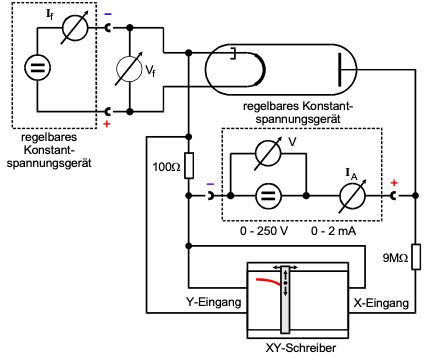
\includegraphics[width=0.7\textwidth]{content/Bilder/ersterAufbau.png}
    \caption{Schaltbild zur Erstellung einer Kennlinie der Hochvakuum-Diode Q\cite{anleitungV504}.}
    \label{fig:ersteApparatur}
\end{figure}

\subsection{Bestimmung des Anlaufstromgebiets}
Beim zweiten Teil der Durchführung wird das Anlaufstromgebiet der Diode untersucht. Hier wird die 
Schaltung in Abbildung \ref{fig:zweiteApparatur} verwendet. Zunächst wird der Heizstrom auf $2,3\,\unit{\ampere}$
eingestellt. Daraufhin wird die Spannung des Gegenfelds schrittweise erhöht und der jeweilige Anodenstrom notiert. 
Zuletzt wird mit den aufgenommen Daten die Kathodentemperatur sowie die Austrittsarbeit bestimmt.
\begin{figure}[H]
    \centering
    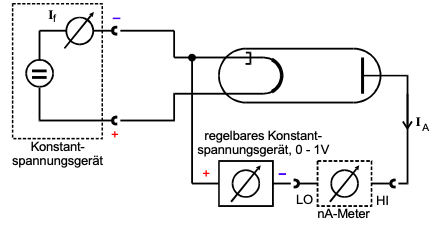
\includegraphics[width=0.7\textwidth]{content/Bilder/zweiterAufbau.png}
    \caption{Schaltbild zur Aufnahme einer Anlaufstromkurve Q\cite{anleitungV504}.}
    \label{fig:zweiteApparatur}
\end{figure}
